\documentclass{article}

% Useful packages
\usepackage[dutch]{babel} % Nederlands taalpakket
\usepackage{multicol}
\setlength{\columnsep}{1cm}

% Set page size and margins
% Replace `letterpaper' with `a4paper' for UK/EU standard size
\usepackage[a4paper,top=2cm,bottom=2cm,left=2cm,right=2cm,marginparwidth=1.75cm]{geometry}

\usepackage{amsmath}
\usepackage{siunitx}
\usepackage{wrapfig}
\usepackage{float}
\usepackage{graphicx}
\graphicspath{{images/}}
\usepackage{subcaption}
\usepackage[colorlinks=true, allcolors=blue]{hyperref}
\usepackage{xcolor}
\usepackage{listings}
\usepackage{import}
\usepackage{xcolor}
\usepackage[toc,page]{appendix} % Pakket voor het maken van bijlagen
\usepackage{hyperref} % Pakket voor hyperlinks en verwijzingen
\usepackage{rotating}
\usepackage{array}
\usepackage{multirow}
\usepackage{lscape}
\usepackage{pdflscape}
\usepackage{longtable} % Add the longtable package to define the longtable environment
\usepackage{caption} % Add the caption package to use the \caption command
\usepackage{etex} % Add the etex package to use the \reserveinserts command


% Definieer de kleuren voor syntax highlighting
\definecolor{codegreen}{rgb}{0,0.6,0}
\definecolor{codegray}{rgb}{0.5,0.5,0.5}
\definecolor{codepurple}{rgb}{0.58,0,0.82}
\definecolor{backcolour}{rgb}{0.95,0.95,0.92}



\lstdefinestyle{mystyle}{
    backgroundcolor=\color{backcolour},
    commentstyle=\color{codegreen},
    keywordstyle=\color{codepurple},
    numberstyle=\tiny\color{codegray},
    basicstyle=\footnotesize\ttfamily,
    breakatwhitespace=false,
    breaklines=true,
    captionpos=b,
    keepspaces=true,
    numbers=left,
    numbersep=5pt,
    showspaces=false,
    showstringspaces=false,
    showtabs=false,
    tabsize=2
}

\usepackage[dutch]{babel}% Language setting


\title{
    Life Cycle Engineering \\
    \large Uitvoeren van safety/reliability analyse}

\author{
  Vollmuller, Michel\\
  1809572\\
  \texttt{michel.vollmuller@student.hu.nl}
} 

\begin{document}
\maketitle

% \begin{abstract}
% \end{abstract}

\tableofcontents

\setlength{\parindent}{0pt} % No indentation for new paragraphs

\newpage
\section{Opdracht}
\subsection{Inleiding}
In deze opdracht gaan we dieper in op het analyseren van technische objecten met als doel correctieve en preventieve maatregelen te identificeren om de prestaties te verbeteren en storingen te verminderen. Je zult verschillende technieken toepassen, zoals het opstellen van een functioneel schema, het uitvoeren van een FMEA/FTA (Fault Tree Analysis/Failure Mode and Effects Analysis), en het uitvoeren van een Pareto analyse.

\subsection{Doel}
Het doel van deze opdracht is om studenten vertrouwd te maken met diverse tools en methoden voor het analyseren van technische systemen, met de nadruk op het identificeren van oorzaken van storingen en het verbeteren van prestaties.

\subsection{Opdracht}
\begin{enumerate}
  \item Selectie van de opdracht
  \item Functioneel schema
  \item FMEA/FTA
  \item Pareto analyse
\end{enumerate}

Deze opdracht biedt studenten de mogelijkheid om praktijkervaring op te doen met het analyseren van technische systemen en het toepassen van troubleshooting technieken. Het bevordert ook het vermogen om gegevens te interpreteren, oorzaken te identificeren en oplossingen voor te stellen, wat essentiële vaardigheden zijn in diverse technische disciplines.


\newpage

\section{Functioneel Schema}
\subsection{Inleiding}
Een functioneel schema is een schematische weergave van de werking van een technisch systeem. Een functioneel schema toont de verschillende componenten van het systeem en hun onderlinge relaties. Het doel van een functioneel schema is om een overzicht te geven van de werking van het systeem en de interactie tussen de verschillende componenten. Dit kan helpen bij het identificeren van storingen en het verbeteren van de prestaties van het systeem. In deze sectie zullen we een functioneel schema opstellen voor de Creality Ender 3 V2 3D-printer.

\subsection{Categorieën}
De Creality Ender 3 V2 3D-printer is een populaire 3D-printer die wordt gebruikt voor het maken van driedimensionale objecten door laag voor laag materiaal toe te voegen. Het systeem bestaat uit verschillende componenten die samenwerken om het printproces te voltooien. Binnen de context van een functioneel schema kunnen we de volgende categorieën onderscheiden:
\begin{itemize}
  \item Ingang
  \item Signal Processing
  \item Uitgang
  \item Voeding
  \item User interface
\end{itemize}

Binnen deze categorieën kunnen we de verschillende componenten van de 3D-printer identificeren en hun onderlinge relaties beschrijven. Dit zal ons helpen om een beter begrip te krijgen van de werking van de 3D-printer. De verschillende relaties zijn aangeduid met pijlen die de richting van de gegevensstroom aangeven. De pijlen zijn met kleurcodering aangegeven om de verschillende categorieën te onderscheiden.

\subsection{Onderdelen}
\textbf{Ingang}
\begin{itemize}
  \item End Switches\\
  Hiervan zitten er 2 op de Creality Ender 3 V2, een voor de X-as en een voor de Y-as. Deze worden gebruikt om de printer te kalibreren en de positie van de nozzle te bepalen.
  \item Bed Temperatuur\\
  Dit is een thermistor die de temperatuur van het heated bed meet. Dit is belangrijk voor het printproces, omdat de temperatuur van het bed van invloed is op de hechting van het filament. Wat directe invloed heeft op de kwaliteit van de print.
  \item Nozzle Temperatuur\\
  Dit is een thermistor die de temperatuur van de hotend meet. Dit is belangrijk voor het printproces, omdat de temperatuur van de hotend van invloed is op het smelten van het filament. Wat directe invloed heeft op de kwaliteit van de print.
  \item Probe\\
  Dit is een sensor die de hoogte van het bed meet. Dit is belangrijk voor het printproces, omdat de hoogte van het bed van invloed is op de hechting van het filament. De probe word voornamelijk gebruikt voor het automatisch levelen van het bed in het calibratie proces.
\end{itemize}

\textbf{Signal Processing}
\begin{itemize}
  \item Moeder Board\\
  Dit is het brein van de 3D-printer. Het moederbord ontvangt de signalen van de verschillende sensoren en stuurt de motoren en heaters aan. Het moederbord bevat ook de firmware die de printer aanstuurt.
\end{itemize}

\textbf{Uitgang}
\begin{itemize}
  \item Stepper motor X\\
  Dit is de motor die de X-as van de printer aanstuurt. De motor beweegt de nozzle horizontaal over het printbed.
  \item Stepper motor Y\\
  Dit is de motor die de Y-as van de printer aanstuurt. De motor beweegt het printbed horizontaal onder de nozzle.
  \item Stepper motor Z\\
  Dit is de motor die de Z-as van de printer aanstuurt. De motor beweegt het printbed verticaal omhoog en omlaag. Hiervan zijn er 2, een voor de linker en een voor de rechter kant van de arm waar X-as over beweegt.
  \item Heated Bed\\
  Dit is het verwarmde bed waarop het object wordt geprint. Het heated bed wordt verwarmd om de hechting van het filament te verbeteren.
  \item Hotend\\
  Dit is het verwarmde uiteinde van de printer waar het filament wordt gesmolten. Het hotend is verantwoordelijk voor het extruderen van het filament en het vormen van het object.
  \item Hotend Fan\\
  Dit is de ventilator die het geëxtrudeerde filament koelt zodat het snel hard word en niet meer kan vervormen.
\end{itemize}

\textbf{Voeding}
\begin{itemize}
  \item Power Supply
  De power supply converteert de netspanning naar de benodigde spanning voor de verschillende componenten van de printer.
\end{itemize}

\textbf{User interface}
\begin{itemize}
  \item Display
  Het display is het scherm waarop de gebruiker de printer kan bedienen en de status van het printproces kan volgen. Dit is de enigste plek waar de gebruiker interactie heeft met de printer.
\end{itemize}

\subsection{FMEA Schema}
\begin{figure}[H]
  \centering
  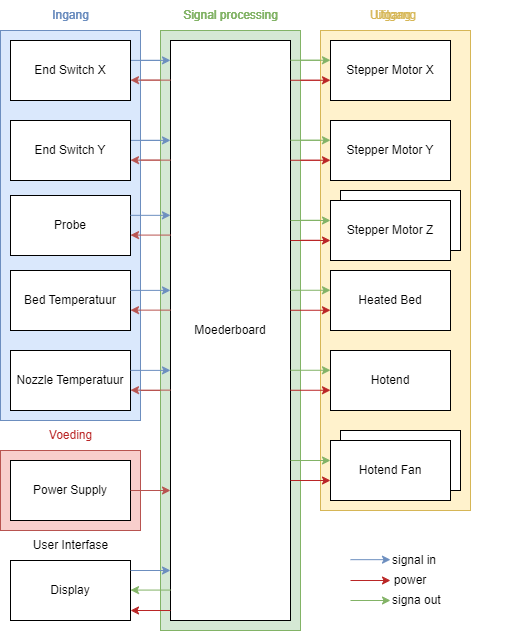
\includegraphics[width=\textwidth]{Creality Ender V2.drawio.png}
\end{figure}


\newpage

\section{FMEA}
\subsection{scope}
\subsection{Onderdelen}
\subsubsection*{End Switches}
% \cite{reddit_end_switches}

\subsubsection*{Bed Temperatuur}
% \cite{reddit_limit_switches}

\newpage
\begin{landscape}
    \subsection{FMEA Table} 
    \begin{longtable}{|l|l|l|c|c|c|c|l|}
        \hline
        \textbf{Item/Functie} & \textbf{Failure mode} & \textbf{Effect} & \textbf{Severity} & \textbf{Occurrence} & \textbf{Detection} & \textbf{RPN} & \textbf{Corr. Action} \\ \hline
        \multirow{3}{*}{Power Supply}       & Defect            & Geen voeding  & 2 & 2 & 5 & 20 & \\
                                            & Kortsluiting      & Geen voeding  & 2 & 2 & 1 &  4 & \\
                                            & Onderbreking      & Geen voeding  & 3 & 2 & 5 & 30 & TE HOOG \\
                                            \hline
        \multirow{4}{*}{End Switch X}       & Sensor defect     & X Switch low  & 2 & 2 & 5 & 20 & \\
                                            & Geen voeding      & X Switch low  & 2 & 2 & 1 &  4 & \\
                                            & false true        & X Switch high & 3 & 2 & 5 & 30 & TE HOOG \\
                                            & false false       & X Switch low  & 2 & 2 & 4 & 16 & \\ 
                                            \hline
        \multirow{4}{*}{End Switch Y}       & Sensor defect     & Y Switch low  & 2 & 2 & 5 & 20 & \\
                                            & Geen voeding      & Y Switch low  & 2 & 2 & 1 &  4 & \\
                                            & false true        & Y Switch high & 3 & 2 & 5 & 30 & TE HOOG \\
                                            & false false       & Y Switch low  & 2 & 2 & 4 & 16 & \\ 
                                            \hline
        \multirow{4}{*}{Probe}              & Sensor defect     & Probe low  & 2 & 2 & 5 & 20 & \\
                                            & Geen voeding      & Probe low  & 2 & 2 & 1 &  4 & \\
                                            & false true        & Probe high & 3 & 2 & 5 & 30 & TE HOOG \\
                                            & false false       & Probe low  & 2 & 2 & 4 & 16 & \\ 
                                            \hline
        \multirow{4}{*}{Bed Temperatuur}    & Sensor defect     & Bed Temperatuur low  & 2 & 2 & 5 & 20 & \\
                                            & Geen voeding      & Bed Temperatuur low  & 2 & 2 & 1 &  4 & \\
                                            & false true        & Bed Temperatuur high & 3 & 2 & 5 & 30 & TE HOOG \\
                                            & false false       & Bed Temperatuur low  & 2 & 2 & 4 & 16 & \\ 
                                            \hline
        \multirow{4}{*}{Nozzle Temperatuur} & Sensor defect     & Nozzle Temperatuur low  & 2 & 2 & 5 & 20 & \\
                                            & Geen voeding      & Nozzle Temperatuur low  & 2 & 2 & 1 &  4 & \\
                                            & false true        & Nozzle Temperatuur high & 3 & 2 & 5 & 30 & TE HOOG \\
                                            & false false       & Nozzle Temperatuur low  & 2 & 2 & 4 & 16 & \\ 
                                            \hline          
        \multirow{3}{*}{Display}            & Defect            & Geen display  & 2 & 2 & 5 & 20 & \\ 
                                            & Kortsluiting      & Geen display  & 2 & 2 & 1 &  4 & \\
                                            & Onderbreking      & Geen display  & 3 & 2 & 5 & 30 & TE HOOG \\
                                            \hline 
        \newpage
        \hline
        \textbf{Item/Functie} & \textbf{Failure mode} & \textbf{Effect} & \textbf{Severity} & \textbf{Occurrence} & \textbf{Detection} & \textbf{RPN} & \textbf{Corr. Action} \\ \hline
        \multirow{15}{*}{Moeder Board}      & Defect                    & printer werkt niet        & 2 & 2 & 5 & 20 & \\
                                            & Geen voeding              & printer werkt niet        & 2 & 2 & 4 & 16 & \\
                                            & X Switch low              & X Stepper rotating        & 2 & 2 & 1 &  4 & \\
                                            & X Switch high             & X Stepper stop signal     & 3 & 2 & 5 & 30 & \\
                                            & Y Switch low              & Y stepper rotating        & 2 & 2 & 1 &  4 & \\
                                            & Y Switch high             & Y stepper stop signal     & 3 & 2 & 5 & 30 & \\
                                            & Probe low                 & Z Stepper rotating        & 2 & 2 & 4 & 16 & \\
                                            & Probe high                & Z Stepper stop signal     & 3 & 2 & 5 & 30 & \\
                                            & Bed Temperatuur low       & Heated Bed heating        & 2 & 2 & 4 & 16 & \\
                                            & Bed Temperatuur high      & Heated Bed not heating    & 3 & 2 & 5 & 30 & \\
                                            & \multirow{2}{*}{Nozzle Temperatuur low}    & Hotend heating            & 2 & 2 & 4 & 16 & \\
                                            &                                            & Hotend Fan standing stil  & 2 & 2 & 4 & 16 & \\
                                            & \multirow{2}{*}{Nozzle Temperatuur high}   & Hotend not heating        & 3 & 2 & 5 & 30 & \\
                                            &                                            & Hotend Fan rotating       & 3 & 2 & 5 & 30 & \\
                                            \hline
        \multirow{4}{*}{Stepper motor X}    & Defect                & Stepper motor not running             & 2 & 2 & 5 & 20 & \\
                                            & No power              & Stepper motor not running             & 2 & 2 & 1 &  4 & \\
                                            & X Stepper rotating    & Stepper motor overheating /burning    & 3 & 2 & 5 & 30 & TE HOOG \\
                                            & X Stepper stop signal & Stepper motor not running             & 2 & 2 & 4 & 16 & \\ 
                                            \hline 
        \multirow{4}{*}{Stepper motor Y}    & Defect                & Stepper motor not running             & 2 & 2 & 5 & 20 & \\
                                            & No power              & Stepper motor not running             & 2 & 2 & 1 &  4 & \\
                                            & Y Stepper rotating    & Stepper motor overheating /burning    & 3 & 2 & 5 & 30 & TE HOOG \\
                                            & Y Stepper stop signal & Stepper motor not running             & 2 & 2 & 4 & 16 & \\ 
                                            \hline
        \multirow{4}{*}{Stepper motor Z}    & Defect                & Stepper motor not running             & 2 & 2 & 5 & 20 & \\
                                            & No power              & Stepper motor not running             & 2 & 2 & 1 &  4 & \\
                                            & Z Stepper rotating    & Stepper motor overheating /burning    & 3 & 2 & 5 & 30 & TE HOOG \\
                                            & Z Stepper stop signal & Stepper motor not running             & 2 & 2 & 4 & 16 & \\ 
                                            \hline 
        \multirow{4}{*}{Heated Bed}         & Defect                    & Bed stays cool, Print wil not stick to the bed    & 2 & 2 & 5 & 20 & \\
                                            & No power                  & Bed stays cool, Print wil not stick to the bed    & 2 & 2 & 1 &  4 & \\
                                            & Heated bed heating        & Heated bed continuously heating, fire             & 3 & 2 & 5 & 30 & TE HOOG \\
                                            & Heated bed not heating    & Bed stays cool, Print wil not stick to the bed    & 2 & 2 & 4 & 16 & \\ 
                                            \hline 
        \multirow{4}{*}{Hotend}             & Defect                    & Hotend stays cool, Filament wil not melt          & 2 & 2 & 5 & 20 & \\
                                            & No power                  & Hotend stays cool, Filament wil not melt          & 2 & 2 & 1 &  4 & \\
                                            & Hotend heating            & Hotend continuously heating, fire                 & 3 & 2 & 5 & 30 & TE HOOG \\
                                            & Hotend not heating        & Hotend stays cool, Filament wil not melt          & 2 & 2 & 4 & 16 & \\ 
                                            \hline
        \multirow{4}{*}{Hotend Fan}         & Defect                    & Hotend Fan not rotating                           & 2 & 2 & 5 & 20 & \\
                                            & No power                  & Hotend Fan not rotating                           & 2 & 2 & 1 &  4 & \\
                                            & Hotend Fan rotating       & Hotend Fan continuously rotating                  & 3 & 2 & 5 & 30 & TE HOOG \\
                                            & Hotend Fan standing stil  & Hotend Fan not rotating, fire                     & 2 & 2 & 4 & 16 & \\ 
                                            \hline   
    \end{longtable}
\end{landscape}


\newpage
\section{Pareto analyse}


\newpage
%Bibliography
% \bibliographystyle{IEEEtran}
% \bibliography{bib}
% \addcontentsline{toc}{section}{Referenties}

% \newpage
% % Bijlage's 
% \appendix 

%   \section{Datasheet RE25 118745}
%     \label{app:datasheet motor}
%     \begin{figure}[htbp]
%       \centering % trim=left bottom right top
%       \includegraphics[page=1, clip, trim=0cm 0cm 0cm 0cm, scale = 0.65]{datasheet_RE25118745.pdf}
%       % \caption{datasheet RE25 118745}
%     \end{figure}
%     \cite{Maxon}


\end{document}